\documentclass[11pt,a4paper]{article}

\usepackage[T1]{fontenc}
\usepackage{lmodern}
\usepackage[a4paper,margin=2.5cm]{geometry}
\usepackage{microtype}
\usepackage{amsmath,amssymb}
\usepackage{graphicx}
\usepackage{booktabs,tabularx,array}
\usepackage{caption}
\usepackage{enumitem}
\usepackage{adjustbox}
\usepackage{xcolor}
\usepackage{fancyhdr}
\usepackage{tikz}
\usetikzlibrary{positioning,arrows.meta}
\usepackage[numbers,sort&compress]{natbib}
\usepackage[colorlinks=true,linkcolor=blue!50!black,citecolor=blue!50!black,urlcolor=blue!50!black]{hyperref}

\graphicspath{{../figures/}}
\newcommand{\ClearEdges}{499}
\newcommand{\Commits}{37}
\newcommand{\DownstreamFirst}{156}
\newcommand{\DroppedTrain}{1\,034}
\newcommand{\Edges}{1\,515}
\newcommand{\FreeFlowMph}{63.2}
\newcommand{\ImpSpeedFifteen}{54.0}
\newcommand{\ImpSpeedSixty}{36.2}
\newcommand{\LongestOutageHours}{31.8}
\newcommand{\LstmGapFifteen}{0.04}
\newcommand{\MaskedTest}{12.12}
\newcommand{\MaskedTrain}{2.96}
\newcommand{\MaskedVal}{6.98}
\newcommand{\NbGainFifteen}{3.5}
\newcommand{\NbGainSixty}{1.4}
\newcommand{\NbGainThirty}{2.6}
\newcommand{\NbGainValFifteen}{4.2}
\newcommand{\NbGainValSixty}{2.5}
\newcommand{\NbGainValThirty}{3.8}
\newcommand{\NbMaeFifteen}{2.91}
\newcommand{\NbMaeSixty}{3.95}
\newcommand{\NbMaeThirty}{3.42}
\newcommand{\NbRmseFifteen}{5.17}
\newcommand{\NbShareFifteen}{4.5}
\newcommand{\NbShareSixty}{7.8}
\newcommand{\NbShareThirty}{6.3}
\newcommand{\NetworkOutagePct}{6.27}
\newcommand{\NetworkOutageSteps}{2\,148}
\newcommand{\NormalXgbFifteen}{2.7}
\newcommand{\NormalXgbSixty}{3.7}
\newcommand{\NormalXgbThirty}{3.1}
\newcommand{\OnsetNbFifteen}{14.42}
\newcommand{\OnsetRatioFifteen}{5.9}
\newcommand{\OnsetRatioSixty}{5.2}
\newcommand{\OnsetRatioThirty}{6.4}
\newcommand{\OnsetReductionFifteen}{11}
\newcommand{\OnsetReductionThirty}{7}
\newcommand{\OnsetSharePct}{2.17}
\newcommand{\OnsetXgbFifteen}{16.2}
\newcommand{\OnsetXgbFifteenTwo}{16.20}
\newcommand{\OnsetXgbSixty}{19.1}
\newcommand{\OnsetXgbThirty}{20.1}
\newcommand{\PctAtLeastSixty}{66.36}
\newcommand{\PeakRatioMax}{1.95}
\newcommand{\PeakRatioMin}{1.42}
\newcommand{\ResidLinkFifteen}{0.12}
\newcommand{\ResidLinkNbSixty}{0.197}
\newcommand{\ResidLinkSixty}{0.20}
\newcommand{\ResidLinkSixtyThree}{0.200}
\newcommand{\ResidTwoSixty}{0.05}
\newcommand{\RowsTest}{1\,416\,501}
\newcommand{\RowsTrain}{4\,747\,131}
\newcommand{\RowsVal}{707\,319}
\newcommand{\ScalerMean}{58.58}
\newcommand{\ScalerStd}{12.82}
\newcommand{\SensorOutagePct}{1.84}
\newcommand{\Sensors}{207}
\newcommand{\ShockwaveKmh}{16}
\newcommand{\TestOnsets}{3\,911}
\newcommand{\TestsTotal}{40}
\newcommand{\Timestamps}{34\,272}
\newcommand{\TwoWayPct}{26.67}
\newcommand{\UpstreamFirst}{41}
\newcommand{\WeakEdgePct}{62.2}
\newcommand{\WindowsTest}{6\,843}
\newcommand{\WindowsTrain}{22\,933}
\newcommand{\WindowsVal}{3\,417}
\newcommand{\XgbAccFifteen}{91.8}
\newcommand{\XgbAccSixty}{88.0}
\newcommand{\XgbAccThirty}{89.9}
\newcommand{\XgbBestDepth}{10}
\newcommand{\XgbHighRoundHorizons}{9}
\newcommand{\XgbNbAccFifteen}{92.3}
\newcommand{\XgbNbAccSixty}{88.3}
\newcommand{\XgbNbAccThirty}{90.4}
\newcommand{\XgbOffpeakFifteen}{2.69}
\newcommand{\XgbOffpeakSixty}{3.32}
\newcommand{\XgbPeakFifteen}{4.22}
\newcommand{\XgbPeakSixty}{6.23}
\newcommand{\XgbRmseFifteenTwo}{5.47}
\newcommand{\XgbVsPersistenceFifteen}{14}
\newcommand{\XgbVsPersistenceSixty}{25}
\newcommand{\XgbWithinFifteen}{84.3}
\newcommand{\XgbWithinSixty}{78.6}
\newcommand{\XgbWithinThirty}{81.4}
\newcommand{\ZeroPct}{8.11}
\newcommand{\histavgMAEFifteen}{4.42}
\newcommand{\histavgMAESixty}{4.42}
\newcommand{\histavgMAEThirty}{4.42}
\newcommand{\histavgMAPEFifteen}{13.9}
\newcommand{\histavgMAPESixty}{13.9}
\newcommand{\histavgMAPEThirty}{13.9}
\newcommand{\histavgPooledMAE}{4.42}
\newcommand{\histavgRMSEFifteen}{8.08}
\newcommand{\histavgRMSESixty}{8.08}
\newcommand{\histavgRMSEThirty}{8.08}
\newcommand{\lstmMAEFifteen}{2.97}
\newcommand{\lstmMAESixty}{4.35}
\newcommand{\lstmMAEThirty}{3.55}
\newcommand{\lstmMAPEFifteen}{8.0}
\newcommand{\lstmMAPESixty}{13.5}
\newcommand{\lstmMAPEThirty}{10.3}
\newcommand{\lstmPooledMAE}{3.54}
\newcommand{\lstmRMSEFifteen}{5.84}
\newcommand{\lstmRMSESixty}{8.84}
\newcommand{\lstmRMSEThirty}{7.19}
\newcommand{\persistenceMAEFifteen}{3.49}
\newcommand{\persistenceMAESixty}{5.37}
\newcommand{\persistenceMAEThirty}{4.20}
\newcommand{\persistenceMAPEFifteen}{8.6}
\newcommand{\persistenceMAPESixty}{14.5}
\newcommand{\persistenceMAPEThirty}{10.8}
\newcommand{\persistencePooledMAE}{4.23}
\newcommand{\persistenceRMSEFifteen}{6.39}
\newcommand{\persistenceRMSESixty}{10.29}
\newcommand{\persistenceRMSEThirty}{8.01}
\newcommand{\rfMAEFifteen}{3.08}
\newcommand{\rfMAESixty}{4.45}
\newcommand{\rfMAEThirty}{3.68}
\newcommand{\rfMAPEFifteen}{8.3}
\newcommand{\rfMAPESixty}{13.5}
\newcommand{\rfMAPEThirty}{10.6}
\newcommand{\rfPooledMAE}{3.64}
\newcommand{\rfRMSEFifteen}{5.61}
\newcommand{\rfRMSESixty}{7.85}
\newcommand{\rfRMSEThirty}{6.71}
\newcommand{\ridgeMAEFifteen}{3.31}
\newcommand{\ridgeMAESixty}{5.17}
\newcommand{\ridgeMAEThirty}{4.08}
\newcommand{\ridgeMAPEFifteen}{8.9}
\newcommand{\ridgeMAPESixty}{15.5}
\newcommand{\ridgeMAPEThirty}{11.7}
\newcommand{\ridgePooledMAE}{4.08}
\newcommand{\ridgeRMSEFifteen}{5.88}
\newcommand{\ridgeRMSESixty}{8.67}
\newcommand{\ridgeRMSEThirty}{7.19}
\newcommand{\xgbMAEFifteen}{3.02}
\newcommand{\xgbMAESixty}{4.01}
\newcommand{\xgbMAEThirty}{3.51}
\newcommand{\xgbMAPEFifteen}{8.2}
\newcommand{\xgbMAPESixty}{12.0}
\newcommand{\xgbMAPEThirty}{10.1}
\newcommand{\xgbPooledMAE}{3.44}
\newcommand{\xgbRMSEFifteen}{5.47}
\newcommand{\xgbRMSESixty}{7.27}
\newcommand{\xgbRMSEThirty}{6.41}


\captionsetup{font=small,labelfont=bf,skip=6pt}
\setlist{itemsep=2pt,topsep=4pt}
\setlength{\parindent}{0pt}
\setlength{\emergencystretch}{2em}
\setlength{\parskip}{6pt}
\renewcommand{\arraystretch}{1.15}
\pagestyle{fancy}
\fancyhf{}
\fancyhead[L]{\small Traffic flow forecasting on METR-LA}
\fancyhead[R]{\small AML project report}
\fancyfoot[C]{\small\thepage}

\newcommand{\dashboard}{\url{https://trafficflowamldl.streamlit.app}}
\newcommand{\repository}{\url{https://github.com/ManasSaxena14/TrafficFlowControl_AIML-DL_T036}}

\title{\vspace{-1cm}\textbf{Traffic Flow Prediction and Signal Control\\via Graph Attention Networks and Flow Models}\\[6pt]
\large Project report: leak-free per-sensor baselines and the measured gap to network-aware learning}
\author{Manas Saxena\\[2pt]\small Applied Machine Learning, Project T036}
\date{\today}

\begin{document}
\maketitle
\thispagestyle{empty}

\begin{center}
\small
Source code and data pipeline: \repository\\
Interactive results dashboard (deployed): \dashboard
\end{center}

\begin{abstract}
\noindent Predicting congestion on a road network is a spatial as well as a temporal problem: a jam forms at a bottleneck and travels backwards along the road, so the most informative signal for a sensor may sit at its neighbours.
This report tests that idea on METR-LA, \Sensors{} freeway sensors in Los Angeles sampled every five minutes, for forecasts 5 to 60 minutes ahead.
We build a leak-free preprocessing pipeline (chronological purged split, outage masking, train-only scaling), six forecasting baselines (persistence, historical average, Ridge, XGBoost, Random Forest and an LSTM without a graph), and four experiments that measure what independent per-sensor models miss.
XGBoost is the strongest independent model, with a test mean absolute error of \xgbMAEFifteen, \xgbMAEThirty{} and \xgbMAESixty{} mph at 15, 30 and 60 minutes.
Its error is \OnsetRatioFifteen{} to \OnsetRatioThirty{} times larger in the 30 minutes after a congestion onset, and the errors of road-linked sensors are correlated (\ResidLinkSixty{} at 60 minutes) while those of unconnected sensors are not.
Adding hand-made neighbour speeds lowers error at every horizon, by up to \NbGainFifteen\% at 15 minutes, which shows that the missing information is spatial but is only partly captured by one-hop features.
All numbers in this report are generated from files in the repository, and a deployed dashboard exposes the same results.
\end{abstract}

\clearpage
\setcounter{tocdepth}{1}
\tableofcontents
\clearpage

%=====================================================================
\section{Introduction}
Road congestion is costly, and forecasting traffic speed a few minutes to an hour ahead is the input to routing, incident response and signal control.
Traffic is a network phenomenon: when a bottleneck saturates, vehicles queue behind it and the slowdown propagates upstream.
A model that forecasts each road segment independently from that segment's own history cannot represent this mechanism, whereas a model that reads the road graph can.
Recent deep-learning work operationalises this with graph neural networks \citep{li2018dcrnn,yu2018stgcn,wu2019graphwavenet}, but the size of the gain over strong per-segment machine-learning baselines, and where it comes from, is rarely isolated under a leak-free protocol.

This project follows a hybrid logic: first build strong segment-level baselines, then identify with evidence what they cannot represent, and only then train a network-aware model.
This report covers the first two stages, the \emph{applied machine learning} (AML) phase.
The graph deep-learning stage is future work and no result for it is claimed here.

\paragraph{Objectives.}
(i)~Build a preprocessing pipeline in which nothing the models are scored on can influence what they are trained on.
(ii)~Implement the baselines named in the project brief (XGBoost per segment or a multi-output Random Forest) and a ladder of simpler and deeper references.
(iii)~Evaluate all models with one shared protocol: chronological splits, equal history windows, MAE, RMSE and MAPE by forecast horizon, and peak versus off-peak.
(iv)~Measure, rather than assert, where independent models fail to capture upstream and downstream propagation.

\paragraph{Contributions.}
\begin{itemize}
  \item A reproducible leak-free pipeline with \TestsTotal{} automated tests, including twelve leakage tests, and a demonstration that a commonly used window-level split lets train and validation targets overlap.
  \item Six baselines scored identically, with test and validation tables at every horizon, an accuracy summary, and a peak versus off-peak breakdown.
  \item Four gap experiments: error against horizon, error after congestion onsets, residual correlation along road links, and a neighbour-information test that bridges per-sensor and graph models.
  \item An open-source repository and a deployed interactive dashboard of all results.
\end{itemize}

\paragraph{Organisation.}
Section~\ref{sec:related} reviews related work, Section~\ref{sec:data} describes the data, Section~\ref{sec:method} the methodology, Sections~\ref{sec:results} and~\ref{sec:gap} the results, Section~\ref{sec:system} the software and deployment, and Sections~\ref{sec:discussion} and~\ref{sec:conclusion} discuss limitations and next steps.

%=====================================================================
\section{Background and related work}\label{sec:related}
\paragraph{Classical and machine-learning forecasting.}
Traffic speed has a strong daily and weekly rhythm, so the historical average per time slot is a standard reference.
Linear models (here Ridge regression, \citealp{hoerl1970ridge}), tree ensembles (Random Forests, \citealp{breiman2001rf}; gradient-boosted trees as implemented in XGBoost, \citealp{chen2016xgboost}) and recurrent networks (LSTM, \citealp{hochreiter1997lstm}) can use lagged speeds and time features, but each treats a sensor as an independent series.

\paragraph{Graph-based deep learning.}
\citet{yu2018stgcn} formulate traffic forecasting on graphs and build the model from fully convolutional structures instead of recurrent units.
\citet{li2018dcrnn} model traffic as a diffusion process on a directed graph and introduce the Diffusion Convolutional Recurrent Neural Network (DCRNN), which captures spatial dependency with bidirectional random walks and temporal dependency with an encoder--decoder trained with scheduled sampling; on METR-LA and PEMS-BAY it improves on the compared baselines by 12\% to 15\%.
\citet{wu2019graphwavenet} learn an adaptive dependency matrix through node embeddings and use stacked dilated one-dimensional convolutions in Graph WaveNet.
Graph attention networks \citep{velickovic2018gat} learn which neighbours matter by attention and are the attention-based option named in the project brief.

\paragraph{Published reference points.}
Table~\ref{tab:published} lists the METR-LA results reported by \citet{li2018dcrnn} next to ours.
They are shown for orientation only: the protocols differ (Section~\ref{sec:protocol}), so the numbers are not directly comparable, and reproducing the published DCRNN under our protocol is the first goal of the next phase.
\begin{table}[ht]
\centering\small
\begin{tabular}{@{}lrrrl@{}}
\toprule
Published (Li et al.) & 15 min & 30 min & 60 min & This work: 15 / 30 / 60 \\
\midrule
Historical average (HA) \cite{li2018dcrnn} & 4.16 & 4.16 & 4.16 & 4.42 / 4.42 / 4.42 \\
FC-LSTM \cite{li2018dcrnn} & 3.44 & 3.77 & 4.37 & 2.97 / 3.55 / 4.35 \\
DCRNN \cite{li2018dcrnn} & 2.77 & 3.15 & 3.60 & not yet built \\
XGBoost (this work) & -- & -- & -- & 3.02 / 3.51 / 4.01 \\
\bottomrule
\end{tabular}

\caption{METR-LA mean absolute error (mph) at 15, 30 and 60 minutes as reported by \citet{li2018dcrnn} (Table~1 of that paper), and ours on the strict test block. Protocols differ; see the text.}
\label{tab:published}
\end{table}

\paragraph{Signal control and simulation.}
The brief also names optional simulated signal control.
Simulators such as CityFlow \citep{zhang2019cityflow} are built for reinforcement-learning research on signal plans. (The brief cites this work as ``Zheng et~al.''; the first author in the proceedings is Huichu Zhang.)
Everything in this project concerning signal control is simulation only; no claim of live traffic control is made.

\paragraph{Research gap addressed here.}
Published graph models are usually compared with older or weaker baselines and under window-level splits.
We therefore ask a narrower, testable question: with a leak-free protocol and strong per-sensor baselines, \emph{where} does an independent model fail, and how much of that is recoverable by giving it neighbour information?
The answer defines the target and the evidence base for the graph models.

%=====================================================================
\section{Data: METR-LA}\label{sec:data}
METR-LA contains speed readings (mph) from loop detectors on Los Angeles County freeways, collected from March to June 2012; we use the version distributed with the DCRNN reference implementation \citep{li2018dcrnn}, whose data originate from \citet{jagadish2014bigdata}.
The sensor graph is the supplied directed adjacency matrix, a thresholded Gaussian kernel of road-network distance.
The order of the speed columns was verified against the adjacency order; this is enforced in code and tested.
\begin{table}[ht]
\centering\small
\begin{tabularx}{\textwidth}{@{}lX@{}}
\toprule
Property & Value \\
\midrule
Sensors and readings & 207 loop detectors; 34\,272 timestamps each \\
Period & 2012-03-01 to 2012-06-27, 5-minute clock, no gaps \\
Readings equal to 0 mph & 8.11\% (6.27 points whole-network, 1.84 points single-sensor) \\
Whole-network outages & 2\,148 timestamps; longest 31.8 h \\
Weekday free-flow speed & 63.2 mph (weekend minimum 56.7 mph) \\
Weekday dips below 90\% of free flow & 07:05--10:45 (low 49.0 mph); 14:30--19:15 (low 45.7 mph) \\
Speed distribution & median 63.22 mph; 66.36\% at least 60 mph; 10.5\% below 40 mph; 2.75\% below 20 mph \\
Road graph & 207 nodes; 1\,515 directed links; mean degree 7.32; 26.67\% two-way; 1 isolated sensor \\
\bottomrule
\end{tabularx}

\caption{Dataset facts (computed in the exploratory analysis, \texttt{results/phase1\_findings.json}).}
\label{tab:dataset}
\end{table}

\subsection{Missing data}
A reading of 0~mph means that the sensor was down, not that traffic stopped (Table~\ref{tab:dataset}).
Of the \ZeroPct\% zero readings, \NetworkOutagePct{} percentage points are whole-network outages (\NetworkOutageSteps{} timestamps at which all sensors are zero, up to \LongestOutageHours{} hours), i.e.\ logging failures, and only \SensorOutagePct{} points are single-sensor failures (Figure~\ref{fig:missing}).
Treating zeros as traffic would teach a model that roads randomly stop, so every later stage masks them.
\begin{figure}[ht]
\centering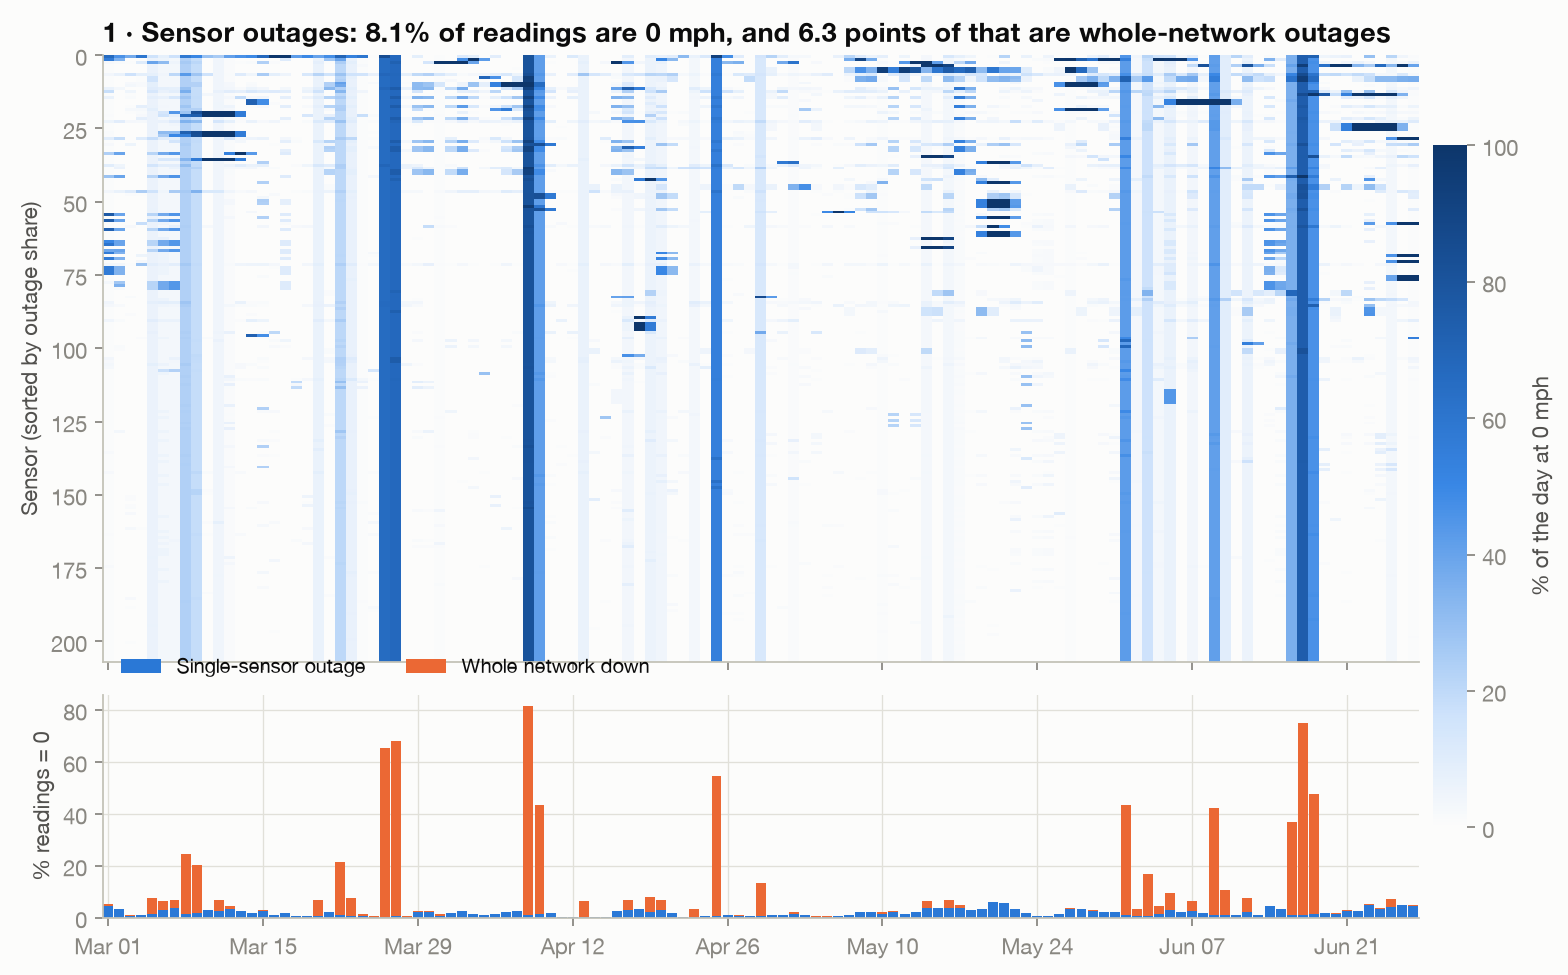
\includegraphics[width=0.92\textwidth]{fig01_missingness.png}
\caption{Share of readings equal to zero by sensor and day, and the part explained by whole-network outages.}
\label{fig:missing}
\end{figure}

\subsection{Daily rhythm}
Weekday speeds dip in the morning and, more deeply, in the afternoon, while weekend speeds stay near free flow (Figure~\ref{fig:profile}).
The brief's peak definition (weekdays 07:00--09:59 and 16:00--19:59) lies inside the detected dips.
Because \PctAtLeastSixty\% of readings are at least 60~mph, average errors are dominated by easy free-flow periods; this motivates reporting peak and congestion-onset results separately.
\begin{figure}[ht]
\centering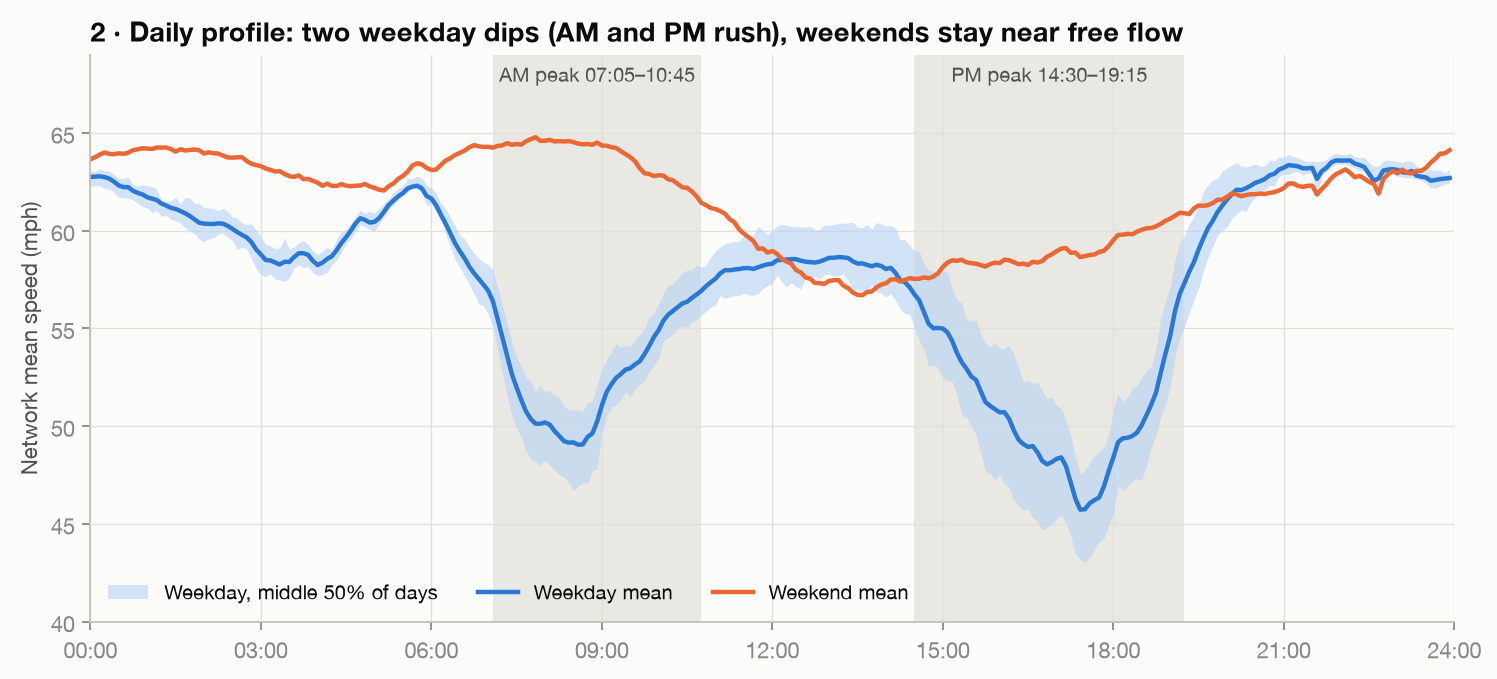
\includegraphics[width=0.92\textwidth]{fig02_daily_profile.png}
\caption{Network-mean speed by time of day for weekdays and weekends (training period only).}
\label{fig:profile}
\end{figure}

\subsection{The road graph and propagation of congestion}\label{sec:propagation}
The graph has \Edges{} directed links, of which only \TwoWayPct\% are two-way, so direction carries information (Figure~\ref{fig:graph}).
To test whether neighbouring sensors carry predictive information, each sensor's typical (weekday-or-weekend and time-slot) pattern was subtracted and the remaining disturbance was cross-correlated along every directed link, using training data only.
\WeakEdgePct\% of links are weak (peak correlation below 0.3).
Among the \ClearEdges{} links with a clear peak, the downstream sensor moves first on \DownstreamFirst{} links and the upstream sensor first on \UpstreamFirst, and the implied backward wave speed is about \ShockwaveKmh~km/h (Figure~\ref{fig:propagation}).
A jam therefore appears at the downstream neighbour before the upstream sensor, which a model that sees only its own history cannot anticipate.
\begin{figure}[ht]
\centering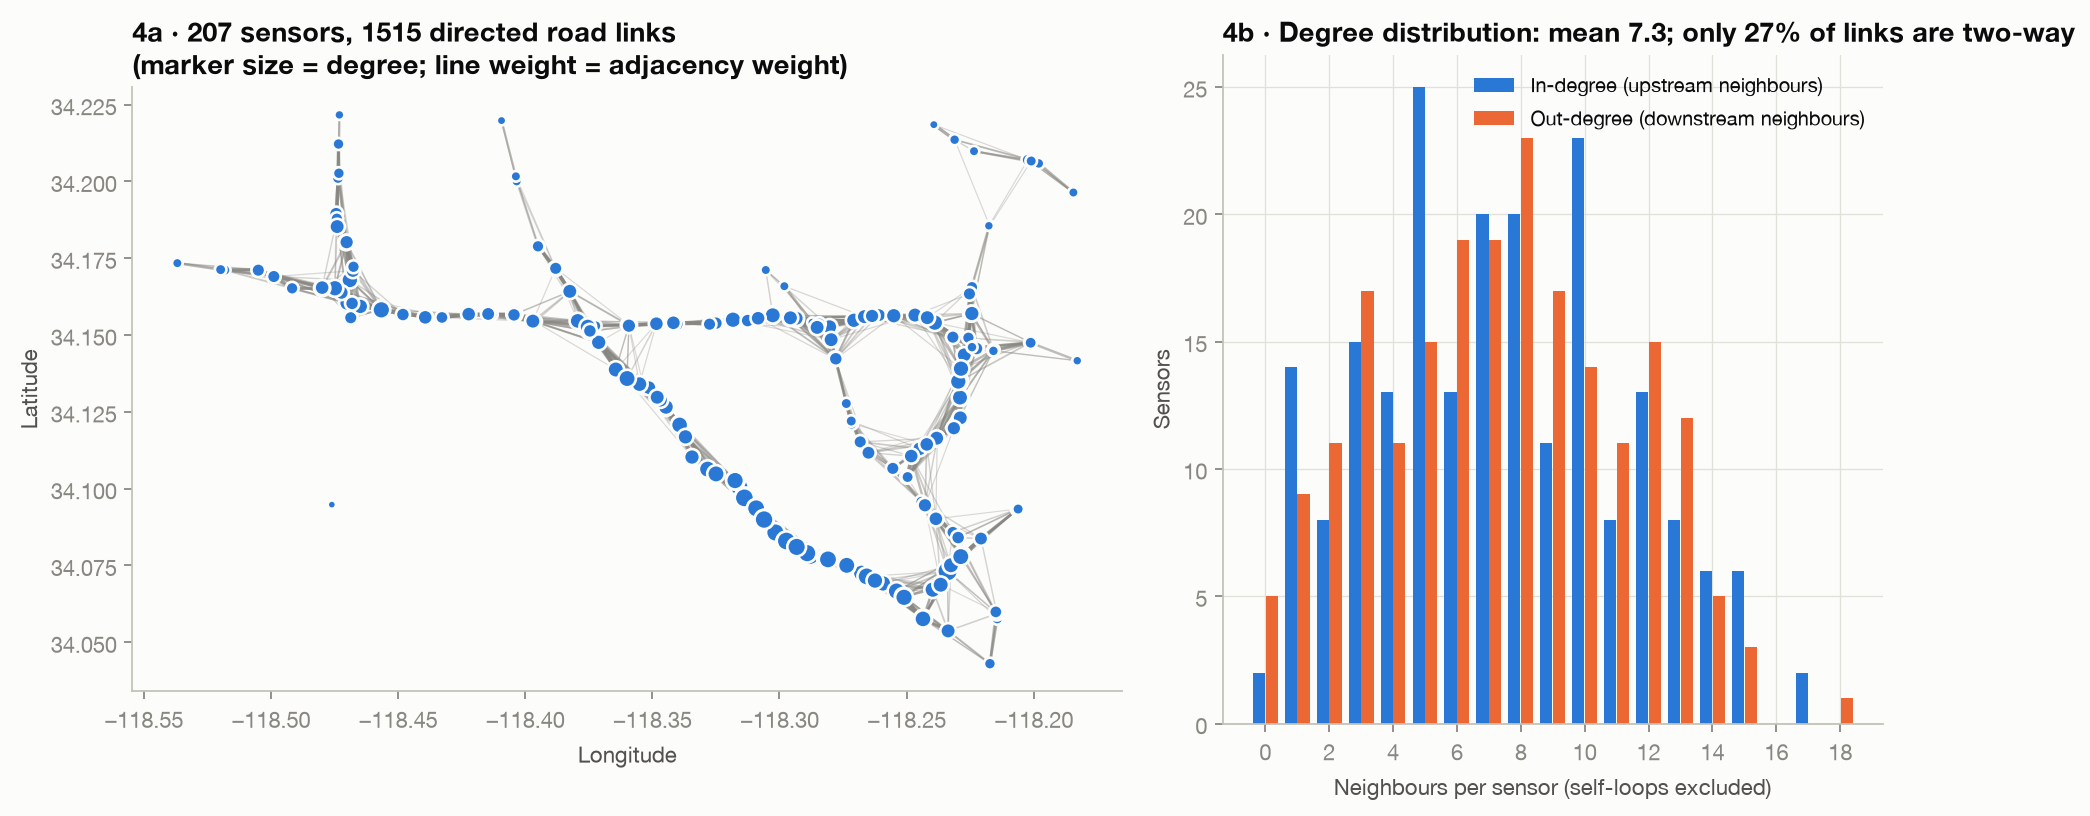
\includegraphics[width=0.78\textwidth]{fig04_sensor_graph.png}
\caption{The sensor graph over Los Angeles (directed links, node size by degree).}
\label{fig:graph}
\end{figure}
\begin{figure}[ht]
\centering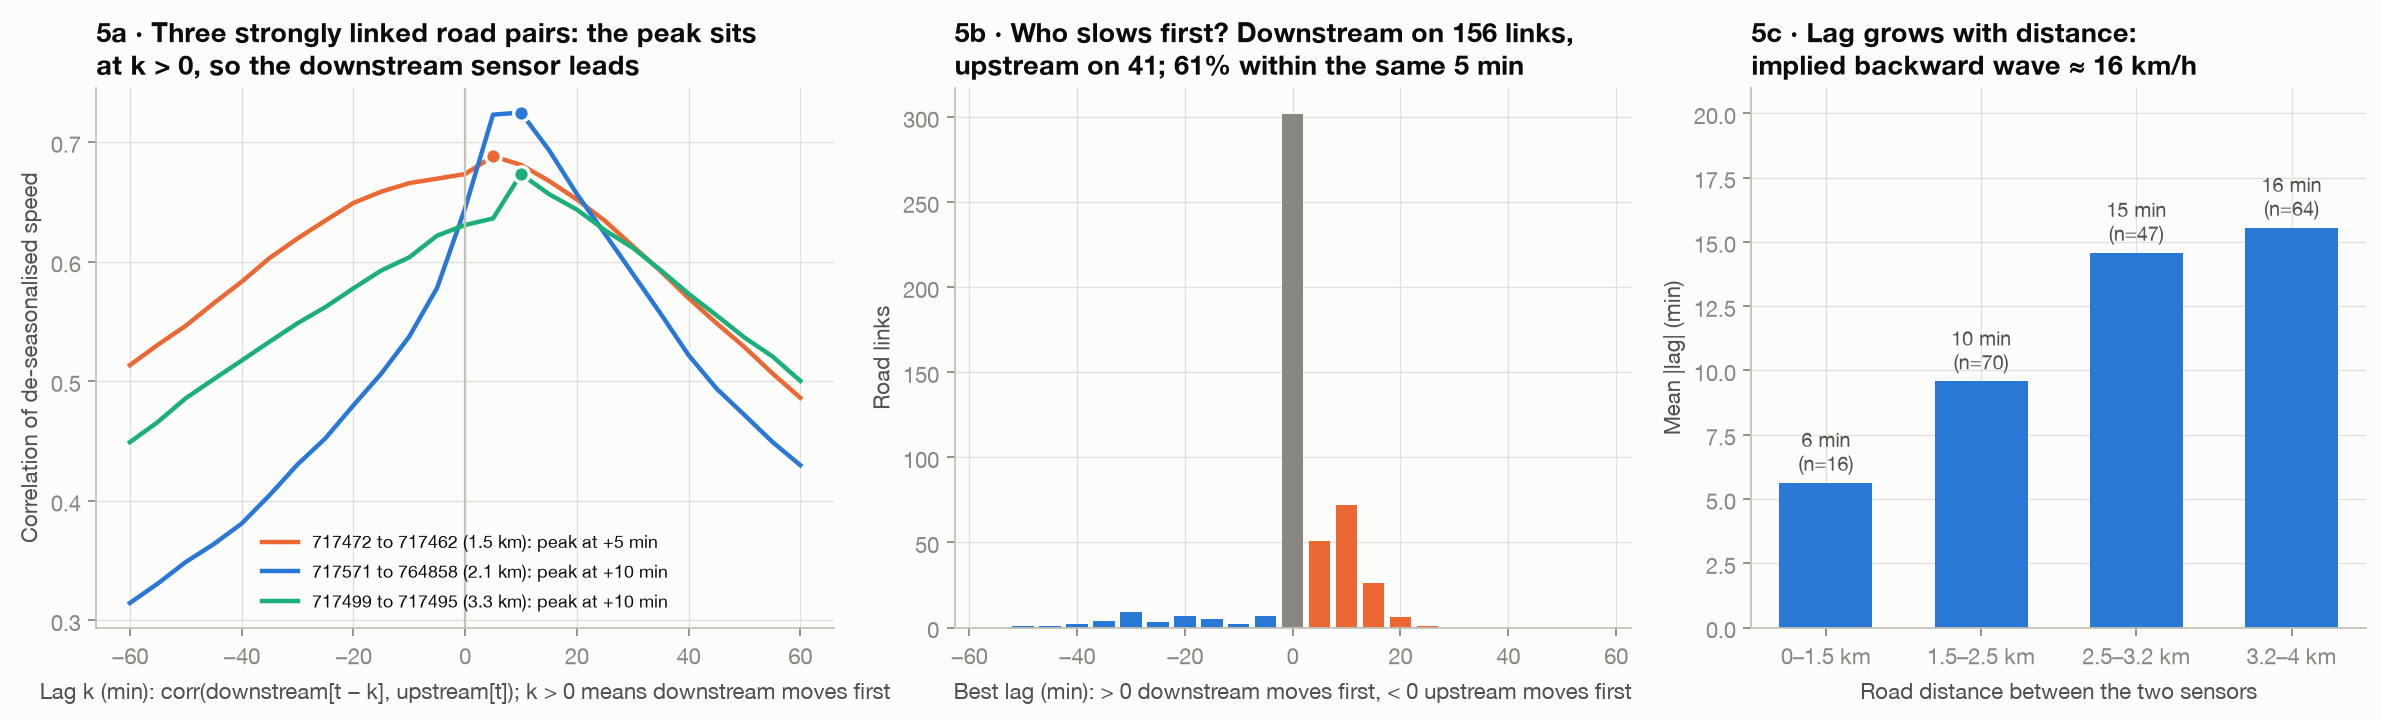
\includegraphics[width=0.92\textwidth]{fig05_spatial_propagation.png}
\caption{Lead--lag analysis along directed links: most strongly coupled links show the downstream sensor moving first, with the lag growing with distance.}
\label{fig:propagation}
\end{figure}
\begin{figure}[ht]
\centering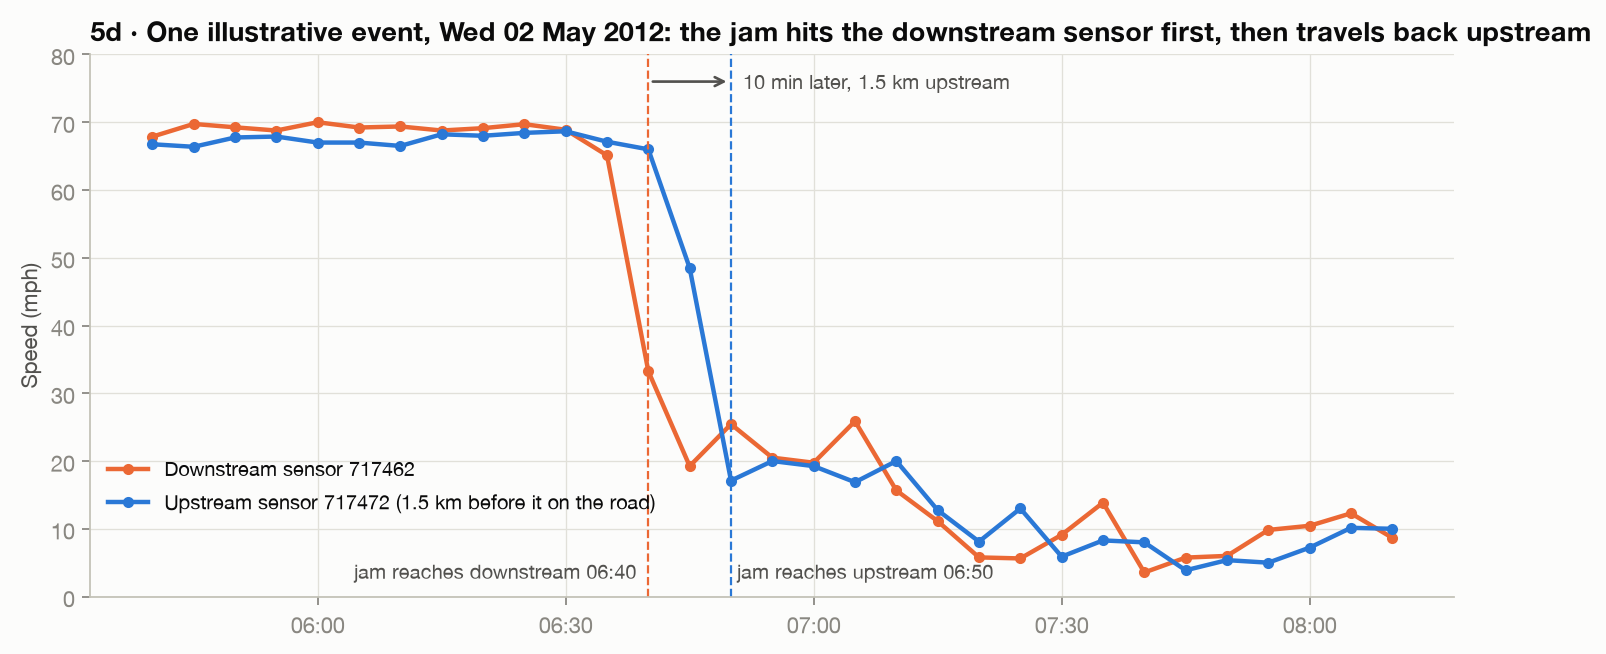
\includegraphics[width=0.92\textwidth]{fig05d_propagation_example.png}
\caption{An illustrative event (2 May 2012): the downstream sensor drops to about 20~mph at 06:40 while the upstream sensor is still at about 66~mph. The event was selected by a rule; the evidence is the all-link statistics above.}
\label{fig:example}
\end{figure}

%=====================================================================
\section{Methodology}\label{sec:method}
\begin{figure}[ht]
\centering
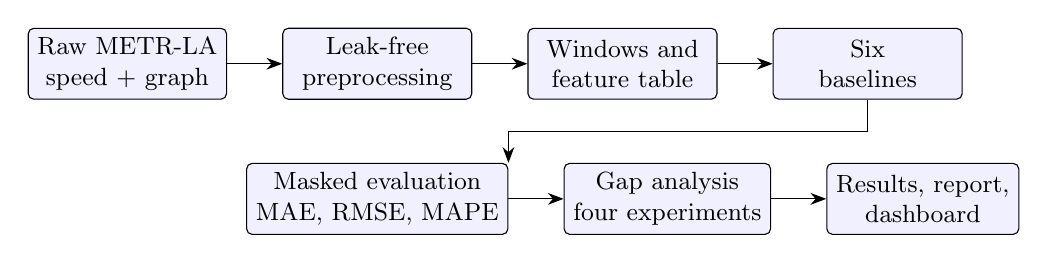
\begin{tikzpicture}[node distance=7mm, every node/.style={font=\small}, box/.style={draw, rounded corners=2pt, align=center, minimum height=9mm, minimum width=24mm, fill=blue!6}, >={Stealth[length=2mm]}]
  \node[box] (raw) {Raw METR-LA\\speed + graph};
  \node[box, right=of raw] (pre) {Leak-free\\preprocessing};
  \node[box, right=of pre] (feat) {Windows and\\feature table};
  \node[box, right=of feat] (mod) {Six\\baselines};
  \node[box, below=8mm of pre] (eval) {Masked evaluation\\MAE, RMSE, MAPE};
  \node[box, right=of eval] (gap) {Gap analysis\\four experiments};
  \node[box, right=of gap] (dash) {Results, report,\\dashboard};
  \draw[->] (raw) -- (pre); \draw[->] (pre) -- (feat); \draw[->] (feat) -- (mod);
  \draw[->] (mod.south) |- ++(0,-4mm) -| (eval.north east);
  \draw[->] (eval) -- (gap); \draw[->] (gap) -- (dash);
\end{tikzpicture}
\caption{Pipeline overview. Every stage is a command in the project's Makefile.}
\label{fig:pipeline}
\end{figure}

\subsection{Problem formulation}
Let $x^{(i)}_t$ be the speed of sensor $i\in\{1,\dots,207\}$ at time step $t$ (5 minutes) and $m^{(i)}_t\in\{0,1\}$ indicate a real reading.
Given the last 12 steps $x^{(i)}_{t-11:t}$ (60 minutes) and time features, the task is to forecast $\hat y^{(i)}_{t+h}$ for $h=1,\dots,12$ (5 to 60 minutes ahead).
Headline results use $h=3,6,12$ (15, 30 and 60 minutes).
All models use exactly this 12-step history.

\subsection{Leak-free preprocessing}\label{sec:protocol}
\paragraph{Chronological split with a purge gap.}
Timestamps are split 70, 10 and 20 percent into train, validation and test blocks.
A window is kept only if all 12 of its target timestamps lie in one block; windows whose targets straddle a boundary are purged (11 per boundary), so no target timestamp is in two splits.
Inputs may look back into earlier data: that is the past, not a label, and matches deployment.
\begin{table}[ht]
\centering\small
\begin{tabular}{@{}lrrllr@{}}
\toprule
Split & Windows & Rows & First target & Last target & Masked targets \\
\midrule
Train & 22\,933 & 4\,747\,131 & 2012-03-01 01:00 & 2012-05-23 07:05 & 2.96\% \\
Val & 3\,417 & 707\,319 & 2012-05-23 07:10 & 2012-06-04 04:45 & 6.98\% \\
Test & 6\,843 & 1\,416\,501 & 2012-06-04 04:50 & 2012-06-27 23:55 & 12.12\% \\
\bottomrule
\end{tabular}

\caption{Strict split: windows, rows (windows $\times$ 207 sensors), target period and share of masked targets. The training block also excludes \DroppedTrain{} windows whose targets are over 90\% masked.}
\label{tab:splits}
\end{table}
Table~\ref{tab:protocols} shows why the purge matters.
Splitting \emph{windows} instead of timestamps, as in the reference DCRNN script, makes the first validation target earlier than the last training target, i.e.\ train and validation targets overlap by 50 minutes; such overlap is a form of the leakage studied by \citet{kaufman2012leakage}.
Both protocols are implemented so published numbers can be compared later; all results here use the strict protocol, and a test proves the overlap exists in the reference protocol and not in ours.
\begin{table}[ht]
\centering\small
\begin{tabular}{@{}lll@{}}
\toprule
 & Strict split (used) & Reference window split \\
\midrule
Split unit & timestamps, then windows & windows \\
Last train target & 2012-05-23 07:05 & 2012-05-23 07:40 \\
First validation target & 2012-05-23 07:10 & \textbf{2012-05-23 06:50} (earlier) \\
Scaler mean / std (mph) & 58.58 / 12.82, outages excluded & 54.41 / 19.49, 0 mph included \\
\bottomrule
\end{tabular}

\caption{Strict timestamp split versus the reference window split.}
\label{tab:protocols}
\end{table}

\paragraph{Outage masking.}
Zeros become missing.
In the inputs, a gap is forward-filled from the last real reading inside the same 12-step window, otherwise from the training mean of that sensor and time-of-day slot, and a mask channel tells the model the value is imputed.
Targets stay missing; every loss and metric ignores them.
Training windows whose targets are over 90\% masked, mostly whole-network outages, are dropped; validation and test keep every window.

\paragraph{Scaling.}
Speeds are standardised as $z=(x-\mu)/\sigma$ with $\mu=\ScalerMean$~mph and $\sigma=\ScalerStd$~mph, computed from training timestamps only with outages excluded.
Predictions are inverse-transformed so that all errors are in mph.

\paragraph{Time features and adjacency.}
Time of day and day of week enter as sine and cosine pairs plus a weekend flag, so that 23:55 and 00:05 are neighbours.
The adjacency is rebuilt from road distances $d_{ij}$ as $W_{ij}=\exp\!\big(-(d_{ij}/\sigma_d)^2\big)$ if this is at least $\kappa=0.1$ and 0 otherwise, with $\sigma_d$ the standard deviation of the finite distances, and is asserted equal to the supplied matrix; it stays directed and fixed.

\subsection{Feature table}
One row is one sensor at one forecast origin: 12 lagged speeds; mean, standard deviation and minimum over the last 3, 6 and 12 steps; two differences (speed now minus 1 and 3 steps earlier); 12 real-reading flags and the count of imputed lags; five time features; and five segment descriptors computed on training data only (sensor id, mean speed, free-flow speed as the 85th percentile, in-degree and out-degree), 46 columns in total.
The split sizes in Table~\ref{tab:splits} give \RowsTrain{} training, \RowsVal{} validation and \RowsTest{} test rows.
Flow and occupancy, which the brief lists, are not recorded in METR-LA; they require PeMS data and are a data limitation rather than omitted work.

\subsection{Models}
Table~\ref{tab:models} lists the six baselines.
XGBoost and the Random Forest are \emph{independent} models: a row contains only one sensor's own history, time and static descriptors and never a neighbour's speed.
The LSTM shares weights across sensors but also sees no neighbour, so it separates the effect of deep learning from the effect of the graph; Adam \citep{kingma2015adam} was used for training.
All hyper-parameters and early stopping use the validation block only.
\begin{table}[ht]
\centering\small
\begin{tabularx}{\textwidth}{@{}clX@{}}
\toprule
Rung & Model & Configuration \\
\midrule
0 & Persistence & Repeats the last (imputed) speed for all 12 horizons. \\
1 & Historical average & Training mean per sensor, weekday-or-weekend and 5-minute slot. \\
2 & Ridge per sensor & One linear model per sensor and horizon (207 $\times$ 12) on the 41 time-varying features, standardised per sensor. Penalty chosen from $\{1, 10, 100, 1000\}$ on validation: 1000 (validation MAE 3.859 to 3.858, so the choice barely matters). \\
3 & XGBoost & One regressor per horizon trained on all sensors stacked, sensor id as a feature, masked targets given weight 0. Maximum depth searched at the 30-minute horizon: 10 gives 3.291, 8 gives 3.342, 6 gives 3.413 validation MAE; depth 10 chosen. Learning rate 0.05, row and column subsample 0.8, up to 600 rounds with early stopping (50) on validation; every 2nd window used. \\
4 & Random Forest & One multi-output forest predicting all 12 horizons: 100 trees, depth 20, minimum leaf 10, 30\% bootstrap samples, 50\% of features per split. Trained on every 6th window keeping rows whose 12 targets are all observed (742\,613 rows); evaluated on every test row with the mask. \\
5 & LSTM, no graph & Two LSTM layers of 64 units, dropout 0.1, one set of weights shared by all 207 sensors; input is each sensor's own $12 \times 7$ window, output 12 horizons. Masked MAE in mph, Adam (learning rate 0.002, halved on plateau), gradient clipping 5, at most 12 epochs. All 12 epochs were used; best validation MAE 3.208. \\
\bottomrule
\end{tabularx}

\caption{The six baselines and their configuration.}
\label{tab:models}
\end{table}

\subsection{Evaluation protocol}
Errors are computed only where the target is a real reading:
\begin{align*}
\mathrm{MAE} &= \frac{\sum m\,|\hat y-y|}{\sum m}, &
\mathrm{RMSE} &= \sqrt{\frac{\sum m\,(\hat y-y)^2}{\sum m}}, &
\mathrm{MAPE} &= 100\,\frac{\sum m\,|\hat y-y|/\max(y,1)}{\sum m},
\end{align*}
with the sums over test windows, sensors and (for a given horizon) the 12-step output.
MAPE is sensitive to small denominators \citep{hyndman2006measures}; the 1~mph floor only guards a pathological reading, as targets are real speeds.
To summarise forecasts in plain terms we also report \emph{percent accuracy} (100 minus MAPE) and the share of forecasts within 5~mph of the true speed.
Peak is weekdays 07:00--09:59 and 16:00--19:59, judged on the timestamp being predicted.
Test numbers are written to the results files but never used to choose anything.

\subsection{Gap-analysis methods}
\paragraph{Congestion onset.}
An onset is a speed drop of more than 20~mph within 15 minutes starting from at least 50~mph (3-step rolling median).
A target is ``after an onset'' if it lies within 30 minutes after one at that sensor; this labels evaluation points only and is never a model input.
\paragraph{Residual correlation.}
For each pair of sensors the correlation of their XGBoost residual series, using only timestamps where both readings are real, is grouped by the number of road links between them.
\paragraph{Neighbour-information test.}
XGBoost is given summaries of a sensor's road neighbours in one or both directions (``upstream'' are sensors with a link into it, ``downstream'' those it links to): the weighted mean neighbour speed now and 5, 15 and 30 minutes ago, the slowest neighbour now, and the largest 15-minute drop among neighbours, i.e.\ 6 features per direction.
The same depth, row thinning and early stopping as the base model are used with no extra tuning, for the 15, 30 and 60 minute horizons only.

%=====================================================================
\section{Results: forecasting baselines}\label{sec:results}
\subsection{Scores on the test block}
Table~\ref{tab:test} reports all three metrics at the three headline horizons; Appendix~\ref{app:horizon} gives every horizon and Appendix~\ref{app:val} the validation scores.
\begin{table}[ht]
\centering\footnotesize\setlength{\tabcolsep}{3.5pt}
\adjustbox{max width=\textwidth}{\begin{tabular}{@{}lrrrrrrrrrr@{}}
\toprule
Model & MAE\,15 & MAE\,30 & MAE\,60 & RMSE\,15 & RMSE\,30 & RMSE\,60 & MAPE\,15 & MAPE\,30 & MAPE\,60 & Pooled \\
\midrule
Persistence & 3.49 & 4.20 & 5.37 & 6.39 & 8.01 & 10.29 & 8.6 & 10.8 & 14.5 & 4.23 \\
Historical average & 4.42 & 4.42 & 4.42 & 8.08 & 8.08 & 8.08 & 13.9 & 13.9 & 13.9 & 4.42 \\
Ridge per sensor & 3.31 & 4.08 & 5.17 & 5.88 & 7.19 & 8.67 & 8.9 & 11.7 & 15.5 & 4.08 \\
Random Forest & 3.08 & 3.68 & 4.45 & 5.61 & 6.71 & 7.85 & 8.3 & 10.6 & 13.5 & 3.64 \\
LSTM (no graph) & \textbf{2.97} & 3.55 & 4.35 & 5.84 & 7.19 & 8.84 & \textbf{8.0} & 10.3 & 13.5 & 3.54 \\
XGBoost & 3.02 & \textbf{3.51} & \textbf{4.01} & \textbf{5.47} & \textbf{6.41} & \textbf{7.27} & 8.2 & \textbf{10.1} & \textbf{12.0} & 3.44 \\
\bottomrule
\end{tabular}
}
\caption{Test scores (MAE and RMSE in mph, MAPE in percent) at 15, 30 and 60 minutes; best in each column in bold. ``Pooled MAE'' averages all 12 horizons.}
\label{tab:test}
\end{table}
XGBoost has the lowest RMSE at all three horizons and the lowest MAE and MAPE at 30 and 60 minutes; its MAE is \xgbMAEFifteen, \xgbMAEThirty{} and \xgbMAESixty{} mph, which is \XgbVsPersistenceFifteen\% lower than persistence at 15 minutes and \XgbVsPersistenceSixty\% lower at 60 minutes, and it has the best pooled MAE (\xgbPooledMAE).
The LSTM has the lowest MAE and MAPE at 15 minutes (\lstmMAEFifteen{} against \xgbMAEFifteen{} mph), a difference of \LstmGapFifteen{} mph from a single training run that should not be over-interpreted.
Persistence is a strong floor at 15 minutes but its MAE grows from \persistenceMAEFifteen{} to \persistenceMAESixty{} mph by 60 minutes.
The historical average ignores the present, so its error is flat (\histavgMAEFifteen{} mph); it beats persistence and Ridge at 60 minutes but not the tree models.
Ridge is competitive at 15 minutes, but its MAPE at 60 minutes (\ridgeMAPESixty\%) is the worst of the six because a linear model extrapolates the recent trend too far.
\begin{figure}[ht]
\centering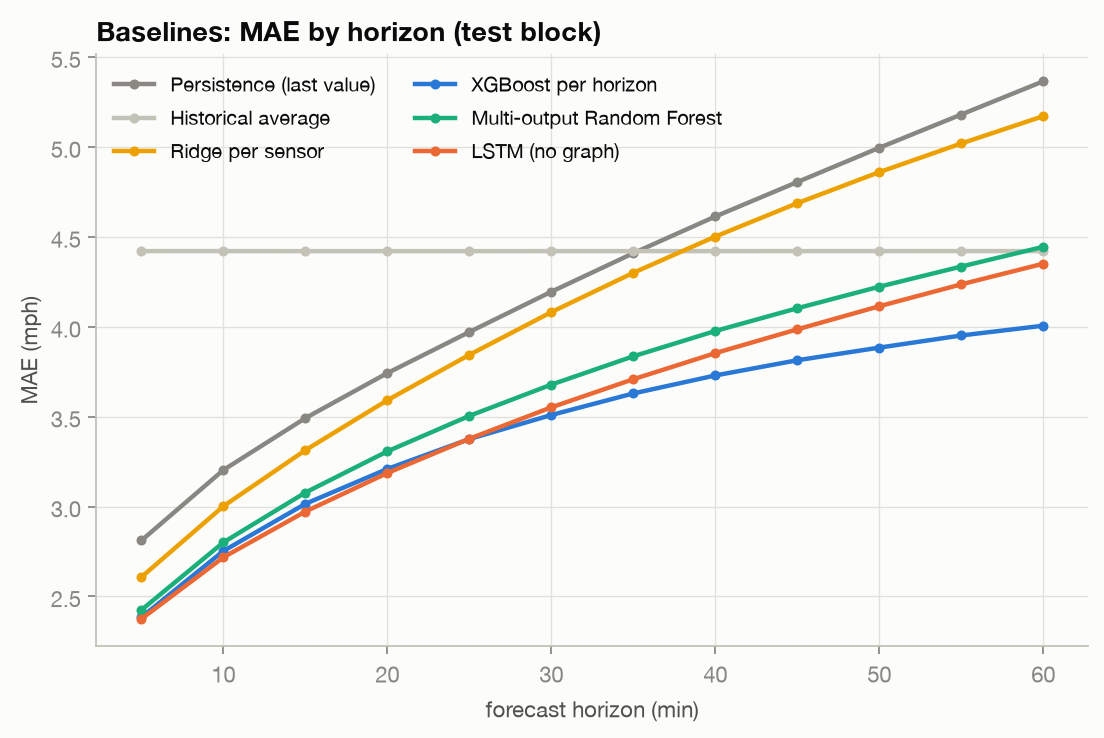
\includegraphics[width=0.85\textwidth]{fig07_baseline_error_by_horizon.png}
\caption{Test MAE by forecast horizon for all six baselines.}
\label{fig:horizon}
\end{figure}

\subsection{Accuracy in plain terms}
Table~\ref{tab:accuracy} converts the errors to percentages.
Speed forecasting is a regression task, so there is no single accuracy figure; percent accuracy and the within-5-mph share are summaries, not formal metrics.
The best independent model is about \XgbAccFifteen\% accurate at 15 minutes, \XgbAccThirty\% at 30 and \XgbAccSixty\% at 60, and \XgbWithinFifteen\% of its 15-minute forecasts are within 5~mph.
These percentages look high mainly because traffic is free-flowing most of the time (even persistence scores about 91\% at 15 minutes), so the error in mph and the error during congestion are the more informative quantities.
\begin{table}[ht]
\centering\small
\begin{tabular}{@{}lrrrrrr@{}}
\toprule
Model & Acc.\,15 & Acc.\,30 & Acc.\,60 & $\leq$5\,mph\,15 & $\leq$5\,mph\,30 & $\leq$5\,mph\,60 \\
\midrule
Persistence & 91.4 & 89.2 & 85.5 & 80.8 & 77.9 & 73.5 \\
Historical average & 86.1 & 86.1 & 86.1 & 76.5 & 76.5 & 76.5 \\
Ridge per sensor & 91.1 & 88.3 & 84.5 & 82.3 & 77.9 & 70.6 \\
Random Forest & 91.7 & 89.4 & 86.5 & 84.1 & 80.6 & 75.9 \\
LSTM (no graph) & 92.0 & 89.7 & 86.5 & 85.1 & 82.6 & 79.5 \\
XGBoost & 91.8 & 89.9 & 88.0 & 84.3 & 81.4 & 78.6 \\
XGBoost + neighbours & 92.3 & 90.4 & 88.3 & 84.7 & 81.7 & 78.8 \\
\bottomrule
\end{tabular}

\caption{Test percent accuracy (``Acc.'', 100 minus MAPE) and share of forecasts within 5~mph, at 15, 30 and 60 minutes.}
\label{tab:accuracy}
\end{table}

\subsection{Peak versus off-peak}
Peak-hour error is \PeakRatioMin{} to \PeakRatioMax{} times the off-peak error across all models and horizons, and the penalty grows with the horizon (Table~\ref{tab:peak}).
XGBoost's weekday-peak MAE rises from \XgbPeakFifteen{} to \XgbPeakSixty{} mph, while its off-peak MAE rises from \XgbOffpeakFifteen{} to \XgbOffpeakSixty{} mph.
Rush hour is when congestion forms and travels, so it is where a network-aware model has the most to gain.
\begin{table}[ht]
\centering\small
\begin{tabular}{@{}llll@{}}
\toprule
Model & Weekday peak & Weekday off-peak & Weekend \\
\midrule
Persistence & 4.61 / 6.05 / 8.32 & 3.25 / 3.74 / 4.62 & 2.86 / 3.31 / 3.98 \\
Historical average & 6.82 / 6.82 / 6.82 & 3.58 / 3.58 / 3.58 & 3.94 / 3.94 / 3.94 \\
Ridge per sensor & 4.58 / 6.02 / 7.93 & 3.00 / 3.56 / 4.40 & 2.71 / 3.27 / 4.10 \\
Random Forest & 4.31 / 5.51 / 7.08 & 2.75 / 3.15 / 3.63 & 2.56 / 3.02 / 3.65 \\
LSTM (no graph) & 4.16 / 5.34 / 6.96 & 2.69 / 3.09 / 3.66 & 2.39 / 2.75 / 3.23 \\
XGBoost & 4.22 / 5.22 / 6.23 & 2.69 / 3.01 / 3.32 & 2.50 / 2.90 / 3.34 \\
\bottomrule
\end{tabular}

\caption{Test MAE (mph) at 15 / 30 / 60 minutes by period.}
\label{tab:peak}
\end{table}

\subsection{What XGBoost relies on}
Table~\ref{tab:importance} and Figure~\ref{fig:importance} show the share of total gain by feature.
The model leans on the current speed and its short-term mean at every horizon (current speed: \ImpSpeedFifteen\% of gain at 15 minutes, \ImpSpeedSixty\% at 60), and as the horizon grows the clock and the sensor's typical speed gain weight.
Nothing in the feature set describes what is happening elsewhere on the network.
\begin{table}[ht]
\centering\small
\begin{tabular}{@{}lrrr@{}}
\toprule
Feature & 15 min & 30 min & 60 min \\
\midrule
speed\_t & 54.0\% & 47.4\% & 36.2\% \\
mean\_3 & 29.7\% & 26.9\% & 21.9\% \\
speed\_t-1 & 3.8\% & 3.4\% & 2.5\% \\
mean\_6 & 2.6\% & 3.0\% & 2.7\% \\
cos\_tod & 1.3\% & 3.0\% & 7.1\% \\
sensor\_mean & 1.1\% & 2.7\% & 6.6\% \\
mean\_12 & 0.9\% & -- & -- \\
sin\_tod & 0.9\% & 2.1\% & 4.8\% \\
free\_flow\_p85 & -- & 1.2\% & 2.5\% \\
\bottomrule
\end{tabular}

\caption{Share of XGBoost's total gain by feature (top eight per horizon; ``--'' means outside the top eight).}
\label{tab:importance}
\end{table}
\begin{figure}[ht]
\centering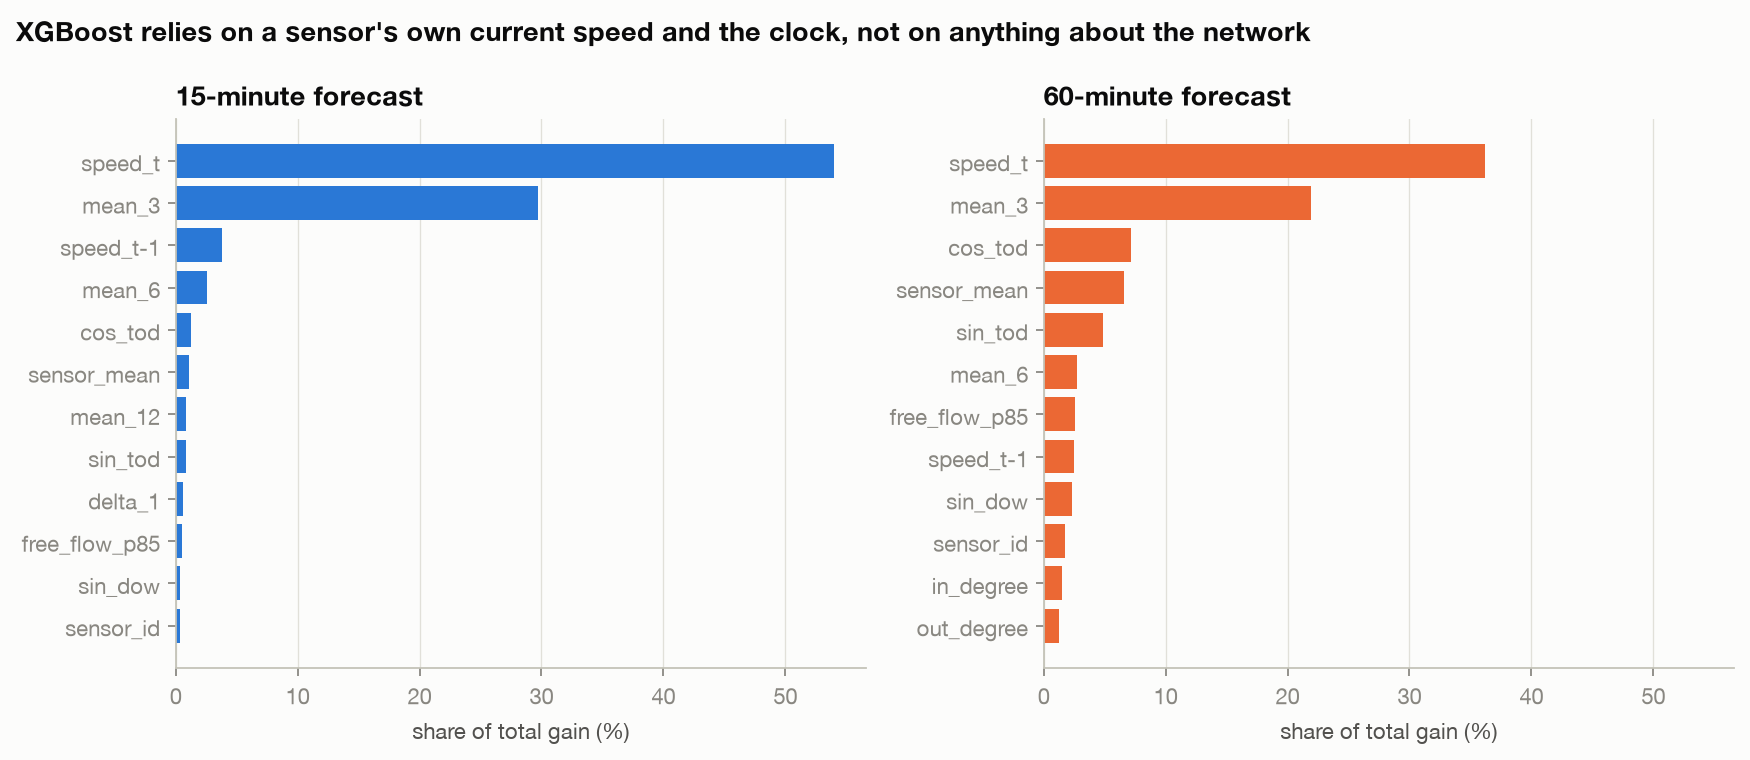
\includegraphics[width=0.92\textwidth]{fig06_xgb_importance.png}
\caption{XGBoost feature importance at 15 and 60 minutes.}
\label{fig:importance}
\end{figure}

%=====================================================================
\section{Results: identifying the gap}\label{sec:gap}
Section~\ref{sec:propagation} showed that congestion propagates between sensors; this section tests whether the best independent model, XGBoost, fails exactly where that matters.
All results use the test block and the saved XGBoost predictions.

\subsection{Error grows steadily with horizon}
XGBoost's MAE rises from \xgbMAEFifteen{} to \xgbMAEThirty{} to \xgbMAESixty{} mph and its RMSE from \xgbRMSEFifteen{} to \xgbRMSEThirty{} to \xgbRMSESixty{} mph (Figure~\ref{fig:gaperr}).
Beyond about 15 minutes the jam that will arrive is not yet visible in the sensor's own history; it is at a neighbour.
\begin{figure}[ht]
\centering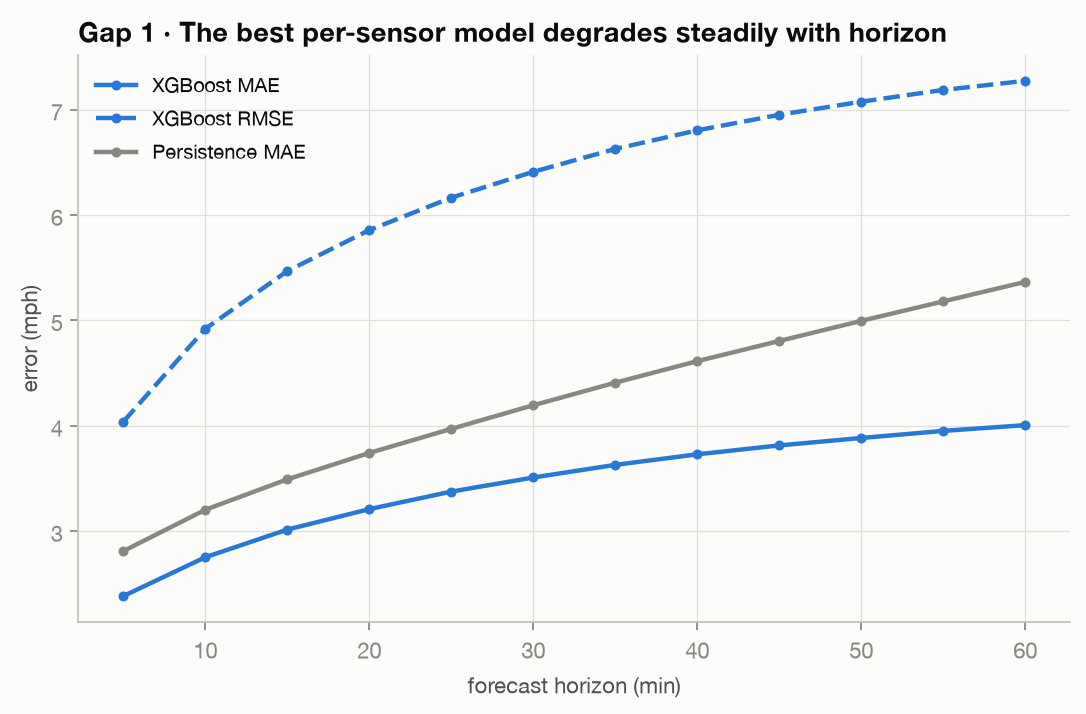
\includegraphics[width=0.78\textwidth]{fig08_gap_error_vs_horizon.png}
\caption{XGBoost error against forecast horizon, with persistence for reference.}
\label{fig:gaperr}
\end{figure}

\subsection{Error after congestion onsets}
The test period contains \TestOnsets{} onsets; the affected targets are \OnsetSharePct\% of all real targets.
In the 30 minutes after an onset, XGBoost's MAE is \OnsetXgbFifteen{} mph at 15 minutes against \NormalXgbFifteen{} mph at other times, a ratio of \OnsetRatioFifteen{}; the ratios at 30 and 60 minutes are \OnsetRatioThirty{} and \OnsetRatioSixty{} (Table~\ref{tab:onset}, Figure~\ref{fig:onset}).
The model keeps forecasting free flow until the slowdown appears in its own lags.
Persistence fails the same way and worse, so the cause is the information available and not the learner.
\begin{table}[ht]
\centering\small
\begin{tabular}{@{}llrrr@{}}
\toprule
Model & Horizon & After onset & Other times & Ratio \\
\midrule
XGBoost & 15 min & 16.20 & 2.72 & 5.9$\times$ \\
XGBoost & 30 min & 20.12 & 3.14 & 6.4$\times$ \\
XGBoost & 60 min & 19.09 & 3.67 & 5.2$\times$ \\
Persistence & 15 min & 17.90 & 3.17 & 5.6$\times$ \\
Persistence & 30 min & 25.35 & 3.73 & 6.8$\times$ \\
Persistence & 60 min & 27.15 & 4.88 & 5.6$\times$ \\
XGBoost + neighbours & 15 min & 14.42 & 2.65 & 5.4$\times$ \\
XGBoost + neighbours & 30 min & 18.77 & 3.08 & 6.1$\times$ \\
XGBoost + neighbours & 60 min & 18.89 & 3.62 & 5.2$\times$ \\
\bottomrule
\end{tabular}

\caption{Test MAE (mph) in the 30 minutes after a congestion onset versus other times.}
\label{tab:onset}
\end{table}
\begin{figure}[ht]
\centering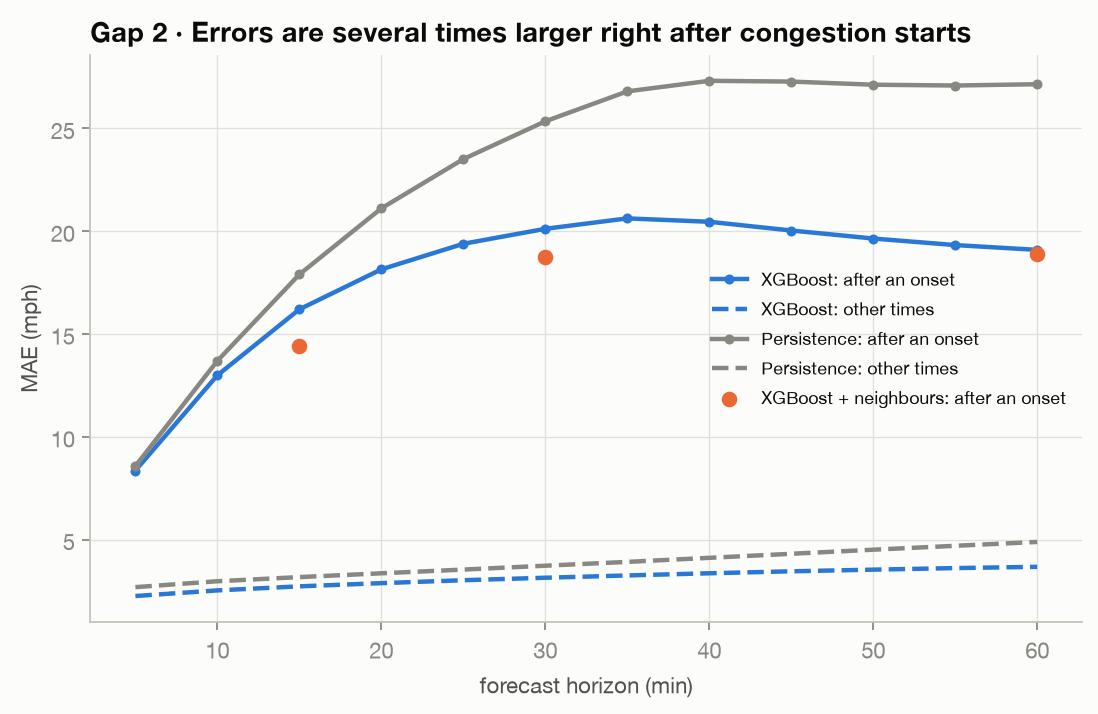
\includegraphics[width=0.78\textwidth]{fig09_gap_onset_error.png}
\caption{MAE after congestion onsets versus other times, by horizon.}
\label{fig:onset}
\end{figure}

\subsection{Errors of linked sensors move together}
Table~\ref{tab:resid} and Figure~\ref{fig:resid} show that the correlation of XGBoost residuals depends on road distance: \ResidLinkSixty{} for sensors one link apart at 60 minutes, \ResidTwoSixty{} for two links and about zero for unconnected sensors.
A network-wide cause such as time of day would also correlate unconnected sensors; it does not.
The correlation grows with horizon (\ResidLinkFifteen{} at 15 minutes to \ResidLinkSixty{} at 60), as expected if the missing information is congestion travelling between sensors.
This is an association, not proof of causation.
\begin{table}[ht]
\centering\small
\begin{tabular}{@{}lrrrr@{}}
\toprule
Pair distance & XGB 15 min & XGB 30 min & XGB 60 min & XGB + nb. 60 min \\
\midrule
1 link & 0.115 & 0.158 & 0.200 & 0.197 \\
2 links & 0.019 & 0.031 & 0.050 & 0.044 \\
3 links & 0.010 & 0.014 & 0.025 & 0.020 \\
4+ links & 0.007 & 0.010 & 0.017 & 0.014 \\
not connected & 0.003 & 0.005 & -0.002 & 0.000 \\
\bottomrule
\end{tabular}

\caption{Mean correlation of residuals between sensor pairs by number of road links (test block). The last column is the neighbour-feature model of Section~\ref{sec:nb}.}
\label{tab:resid}
\end{table}
\begin{figure}[ht]
\centering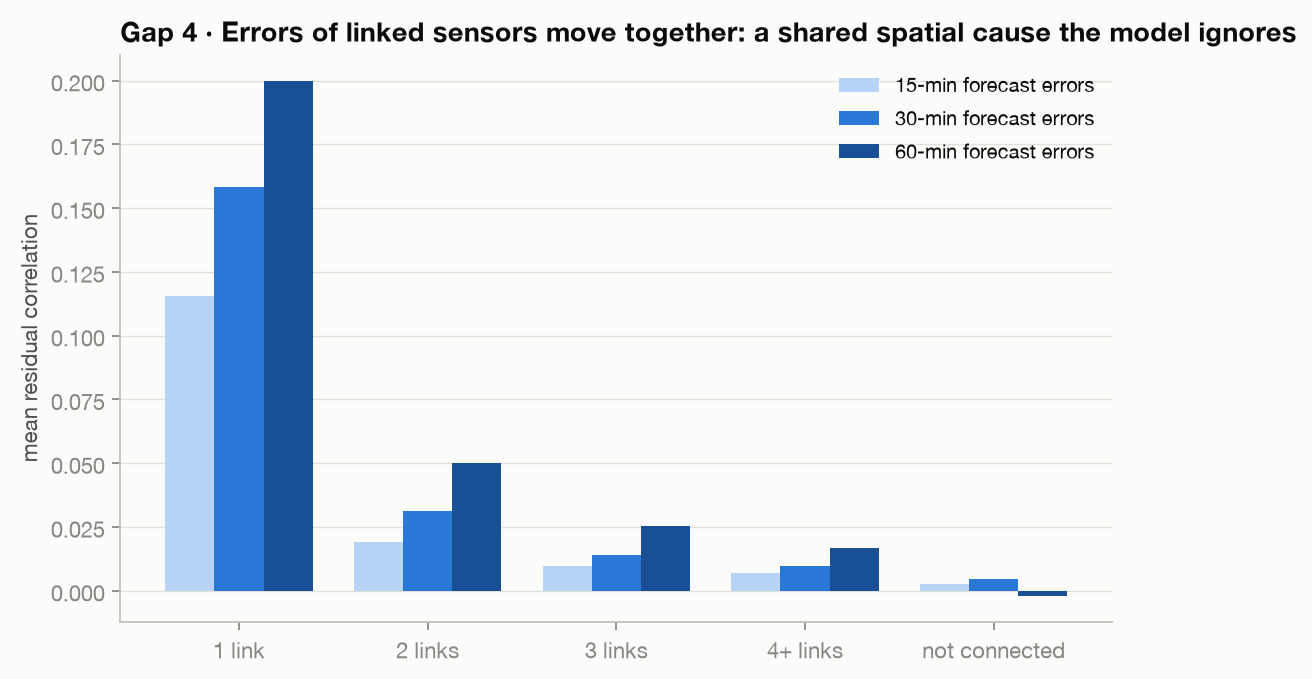
\includegraphics[width=0.78\textwidth]{fig11_gap_residual_correlation.png}
\caption{Residual correlation by road-graph distance.}
\label{fig:resid}
\end{figure}

\subsection{Neighbour-information test}\label{sec:nb}
Table~\ref{tab:nb} and Figure~\ref{fig:nb} give the key experiment.
Every variant beats the independent model at every horizon, and validation shows the same ordering (both directions: $-\NbGainValFifteen$\%, $-\NbGainValThirty$\% and $-\NbGainValSixty$\% MAE).
With both directions, test MAE falls to \NbMaeFifteen, \NbMaeThirty{} and \NbMaeSixty{} mph, i.e.\ by \NbGainFifteen\%, \NbGainThirty\% and \NbGainSixty\%, and RMSE at 15 minutes from \XgbRmseFifteenTwo{} to \NbRmseFifteen{} mph.
Downstream neighbours help more than upstream ones, consistent with the finding that congestion is seen first downstream.
Right after congestion onsets the MAE at 15 minutes falls from \OnsetXgbFifteenTwo{} to \OnsetNbFifteen{} mph (\OnsetReductionFifteen\%) and at 30 minutes by \OnsetReductionThirty\%, a much larger relative gain than the average.
\begin{table}[ht]
\centering\small
\begin{tabular}{@{}lrrrrr@{}}
\toprule
Model & MAE 15 & MAE 30 & MAE 60 & RMSE 15 & MAPE 15 \\
\midrule
XGBoost, own history only & 3.015 & 3.510 & 4.006 & 5.47 & 8.2 \\
+ upstream neighbours & 2.971 (-1.5\%) & 3.472 (-1.1\%) & 3.978 (-0.7\%) & 5.37 & 8.0 \\
+ downstream neighbours & 2.945 (-2.3\%) & 3.461 (-1.4\%) & 3.971 (-0.9\%) & 5.26 & 7.8 \\
+ both directions & 2.908 (-3.5\%) & 3.418 (-2.6\%) & 3.949 (-1.4\%) & 5.17 & 7.7 \\
\bottomrule
\end{tabular}

\caption{Test MAE (mph, change versus own-history XGBoost in brackets) with neighbour features; RMSE (mph) and MAPE (\%) at 15 minutes.}
\label{tab:nb}
\end{table}
\begin{figure}[ht]
\centering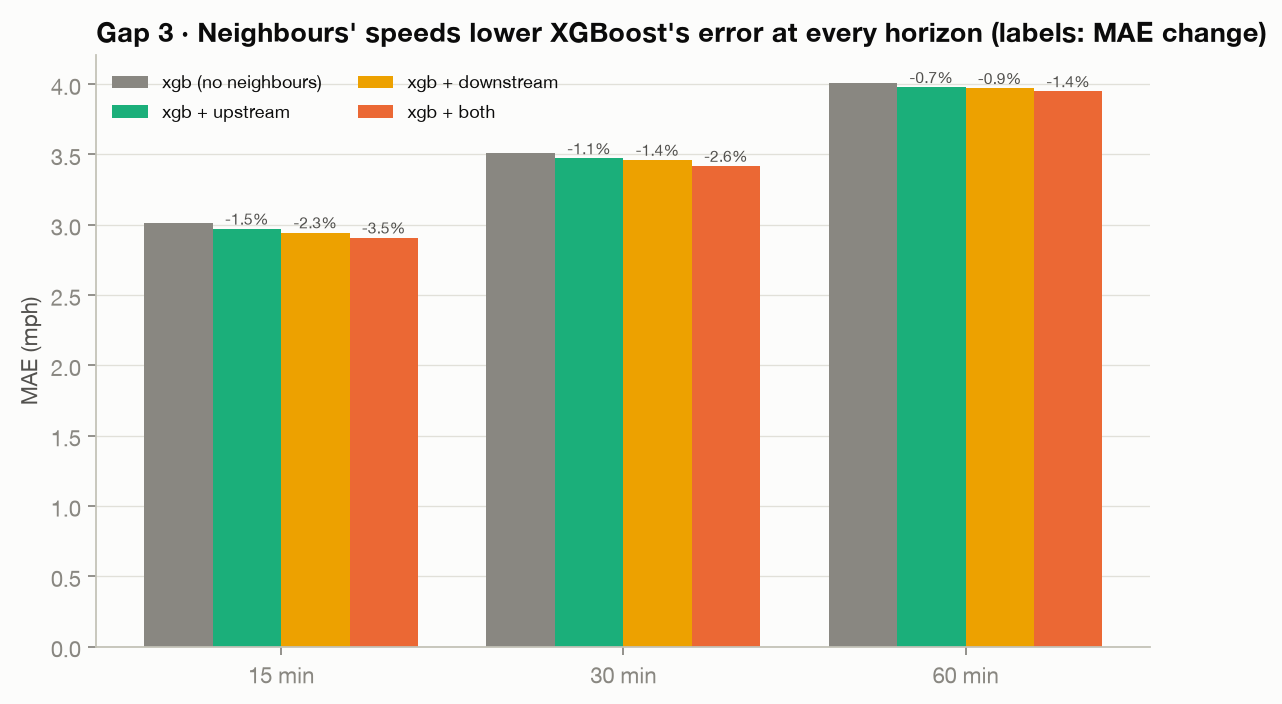
\includegraphics[width=0.78\textwidth]{fig10_gap_neighbour_test.png}
\caption{Test MAE of XGBoost with no, upstream, downstream and both-direction neighbour features.}
\label{fig:nb}
\end{figure}

\paragraph{Why this is not enough.}
The 12 neighbour features together receive only \NbShareFifteen\%, \NbShareThirty\% and \NbShareSixty\% of the model's gain at 15, 30 and 60 minutes.
The gain shrinks at 60 minutes, the residual correlation of linked sensors barely moves (\ResidLinkSixtyThree{} to \ResidLinkNbSixty{} at 60 minutes), and the error after onsets remains several times normal.
A tree model with one-hop summaries cannot learn which neighbour matters when, nor look several links away; this is what attention over the road graph \citep{velickovic2018gat} and multi-hop diffusion \citep{li2018dcrnn} are designed to learn.

\subsection{Gap statement}
\begin{quote}\itshape
Independent segment models forecast each sensor from its own history.
Congestion forms at bottlenecks and travels backwards along road links at about \ShockwaveKmh~km/h, so at longer horizons the most predictive information sits at neighbouring sensors.
We observe this as error rising steadily with horizon, errors \OnsetRatioFifteen{} to \OnsetRatioThirty{} times larger in the 30 minutes after a congestion onset, and residuals correlated only between road-linked sensors.
Handing XGBoost one-hop neighbour summaries lowers error at every horizon but leaves linked residuals correlated and onset errors several times normal.
A graph model that learns which neighbours matter, over several hops, should close this gap.
\end{quote}

%=====================================================================
\section{Software, reproducibility and deployment}\label{sec:system}
\subsection{Repository}
The code is organised as a small Python package with a command for every stage (\repository):
\begin{verbatim}
.
|-- app.py                 Streamlit dashboard (deployed)
|-- Makefile               one command per stage
|-- configs/data/          split, window, masking and peak definitions
|-- src/
|   |-- data/              loading, leak-free preprocessing, readers
|   |-- features/          46-column per-sensor feature table
|   |-- models/            baselines: simple, trees, LSTM
|   |-- eval/              masked metrics, peak evaluation, accuracy
|   |-- analysis/          exploratory analysis and gap analysis
|   |-- train/             runners for baselines and gap experiments
|   `-- viz/               figures
|-- tests/                 automated tests
|-- results/               every result table (CSV and JSON)
|-- notebooks/             exploratory data analysis
|-- scripts/               data download, report table generator
`-- docs/                  this report, figures, slides
\end{verbatim}

\subsection{Testing}
\begin{table}[ht]
\centering\small
\begin{tabularx}{\textwidth}{@{}lrX@{}}
\toprule
Test file & Tests & What it guards \\
\midrule
test\_data.py & 9 & shapes, five-minute clock, sensor order equals graph order, adjacency properties, masking of outages \\
test\_leakage.py & 12 & target order, no target in two splits, train-only scaler, no future inputs, masked metrics, adjacency rebuild \\
test\_baselines.py & 13 & feature alignment, train-only statistics, baselines, tree models, peak labelling, accuracy \\
test\_gap.py & 6 & neighbour direction and features, onset labelling, residual correlation \\
\textbf{Total} & \textbf{40} & all tests pass \\
\bottomrule
\end{tabularx}

\caption{Automated tests.}
\end{table}
The leakage tests check, among others, that target timestamps are ordered and never shared between splits, that the scaler depends only on training data, that altering readings after time $t_0$ does not change any window ending at or before $t_0$, and that masked points contribute exactly zero to the metrics.

\subsection{Reproducing the results}
\texttt{make setup data eda preprocess features baselines gap accuracy test} rebuilds everything from the raw download, and \texttt{make report} regenerates the tables in this document from the result files and compiles it.
Intermediate data (about 2.5~GB per protocol) is not committed.
The repository had \Commits{} commits when this report was built.

\subsection{Interactive dashboard}
A Streamlit application, \texttt{app.py}, presents the saved results in five pages (overview, baseline models, model comparison, spatial gap analysis and an XGBoost deep dive).
It reads only the pre-computed files in \texttt{results/} and does not train or import any model code, so it deploys on Streamlit Community Cloud with the repository's \texttt{requirements.txt}.
The deployed dashboard is available at \dashboard.

%=====================================================================
\section{Discussion and limitations}\label{sec:discussion}
\paragraph{Speed only.}
METR-LA has no flow or occupancy, so the brief's flow and occupancy features are not used; PeMS would supply them.
\paragraph{One city, one season.}
The data are freeway sensors in Los Angeles in 2012, so the results may not transfer to other networks or to signalised urban streets.
\paragraph{Single runs, no significance tests.}
Each model was trained once (seed 42).
Small differences, such as the LSTM against XGBoost at 15 minutes, should not be over-interpreted; significance testing is planned.
\paragraph{Limited tuning budgets.}
XGBoost used at least 580 of its 600 allowed rounds at \XgbHighRoundHorizons{} of 12 horizons, so a larger budget might help slightly, and the LSTM used all 12 epochs with validation error still improving slowly.
XGBoost and the Random Forest were trained on thinned windows, and the neighbour experiment covers three horizons.
\paragraph{Validation and test differ.}
The test period has \MaskedTest\% masked targets against \MaskedVal\% on validation (\MaskedTrain\% in training), so test and validation errors are not directly comparable; the test block was used for reporting only.
\paragraph{Definitions drive the gap analysis.}
Onsets use one threshold definition, and residual correlation shows association, not causation.
\paragraph{No reproduction of published graph models yet.}
Table~\ref{tab:published} is not a like-for-like comparison.
Reproducing the published DCRNN within about 5\% under our protocol is the first gate of the next phase.
\paragraph{Simulation only.}
Signal control, if added, will be evaluated only in a simulator and will not be presented as live traffic control.

%=====================================================================
\section{Conclusions and next steps}\label{sec:conclusion}
We built a leak-free pipeline and six baselines, and showed that XGBoost is the strongest independent model (test MAE \xgbMAEFifteen, \xgbMAEThirty{} and \xgbMAESixty{} mph at 15, 30 and 60 minutes).
Four experiments show that its remaining error concentrates right after congestion starts, at rush hour, and in a form shared between road-linked sensors.
Giving it its neighbours' speeds helps at every horizon, so the missing information is spatial, but hand-made one-hop features capture only part of it.

\paragraph{Next steps.}
(i)~A spatio-temporal graph attention network and a DCRNN \citep{li2018dcrnn} over the fixed directed road graph, with ablations (graph versus no graph, directed versus undirected), evaluated on the same splits, windows, masks and metrics; the targets to beat are XGBoost's \xgbMAEFifteen, \xgbMAEThirty{} and \xgbMAESixty{} mph.
(ii)~A fair comparison with peak and off-peak breakdowns and significance tests over seeds.
(iii)~Congestion maps, an optional simulated signal-control experiment, and extensions such as PeMS flow and occupancy.

\paragraph{Contributions.}
Manas Saxena built the preprocessing pipeline, baselines, gap experiments, report and slides; Harsh Raj set up the project and the exploratory analysis; Sumit contributed the Streamlit dashboard.

%=====================================================================
\bibliographystyle{plainnat}
\bibliography{references}

\appendix
\section{Test MAE at every horizon}\label{app:horizon}
\begin{table}[ht]
\centering\scriptsize
\adjustbox{max width=\textwidth}{\begin{tabular}{@{}lrrrrrrrrrrrr@{}}
\toprule
Model & 5 & 10 & 15 & 20 & 25 & 30 & 35 & 40 & 45 & 50 & 55 & 60 \\
\midrule
Persistence & 2.81 & 3.20 & 3.49 & 3.74 & 3.97 & 4.20 & 4.41 & 4.61 & 4.81 & 5.00 & 5.18 & 5.37 \\
Historical average & 4.42 & 4.42 & 4.42 & 4.42 & 4.42 & 4.42 & 4.42 & 4.42 & 4.42 & 4.42 & 4.42 & 4.42 \\
Ridge per sensor & 2.61 & 3.00 & 3.31 & 3.59 & 3.84 & 4.08 & 4.30 & 4.50 & 4.69 & 4.86 & 5.02 & 5.17 \\
Random Forest & 2.42 & 2.80 & 3.08 & 3.31 & 3.50 & 3.68 & 3.84 & 3.98 & 4.10 & 4.22 & 4.34 & 4.45 \\
LSTM (no graph) & 2.38 & 2.72 & 2.97 & 3.19 & 3.38 & 3.55 & 3.71 & 3.85 & 3.99 & 4.11 & 4.24 & 4.35 \\
XGBoost & 2.38 & 2.75 & 3.02 & 3.21 & 3.38 & 3.51 & 3.63 & 3.73 & 3.81 & 3.88 & 3.95 & 4.01 \\
\bottomrule
\end{tabular}
}
\caption{Test MAE (mph) at forecast horizons of 5 to 60 minutes (column headings in minutes).}
\end{table}

\section{Validation scores}\label{app:val}
\begin{table}[ht]
\centering\footnotesize\setlength{\tabcolsep}{3.5pt}
\adjustbox{max width=\textwidth}{\begin{tabular}{@{}lrrrrrrrrrr@{}}
\toprule
Model & MAE\,15 & MAE\,30 & MAE\,60 & RMSE\,15 & RMSE\,30 & RMSE\,60 & MAPE\,15 & MAPE\,30 & MAPE\,60 & Pooled \\
\midrule
Persistence & 3.22 & 3.82 & 4.79 & 6.02 & 7.52 & 9.59 & 7.8 & 9.8 & 13.0 & 3.85 \\
Historical average & 4.74 & 4.74 & 4.73 & 8.75 & 8.75 & 8.73 & 14.5 & 14.4 & 14.4 & 4.74 \\
Ridge per sensor & 3.11 & 3.85 & 4.91 & 5.58 & 6.83 & 8.26 & 8.4 & 11.0 & 14.6 & 3.86 \\
Random Forest & 2.86 & 3.42 & 4.14 & 5.31 & 6.36 & 7.46 & 7.7 & 9.8 & 12.5 & 3.39 \\
LSTM (no graph) & \textbf{2.73} & \textbf{3.23} & 3.89 & 5.49 & 6.77 & 8.22 & \textbf{7.3} & 9.4 & 12.1 & 3.21 \\
XGBoost & 2.82 & 3.29 & \textbf{3.78} & \textbf{5.19} & \textbf{6.12} & \textbf{6.95} & 7.5 & \textbf{9.4} & \textbf{11.1} & 3.23 \\
\bottomrule
\end{tabular}
}
\caption{Validation scores in the same layout as Table~\ref{tab:test}. The validation block was used only to choose settings and for early stopping.}
\end{table}

\clearpage
\section{Traceability}
Every number in this report is generated by \texttt{scripts/make\_report\_tables.py} from the following files; the only values typed into that script are the published reference numbers of Table~\ref{tab:published}.
\begin{center}\small
\begin{tabularx}{\textwidth}{@{}lX@{}}
\toprule
Content & Source in the repository \\
\midrule
Dataset facts, missing data, graph, propagation & \texttt{results/phase1\_findings.json}, \texttt{docs/figures/fig01}--\texttt{fig05d} \\
Split sizes, masked share, scalers & \texttt{data/processed/} (rebuilt by \texttt{make preprocess}), \texttt{configs/data/metr\_la.yaml} \\
Model configuration & \texttt{results/baselines/*.json}, \texttt{src/models/} \\
Test and validation scores & \texttt{results/baselines.csv}, \texttt{results/baselines/*.csv} \\
Accuracy summaries & \texttt{results/accuracy.csv} \\
Peak versus off-peak & \texttt{results/baselines\_peak.csv} \\
Feature importance & \texttt{results/baselines/xgb\_importance.csv} \\
Onsets and residual correlation & \texttt{results/gap/onset\_vs\_normal.csv}, \texttt{results/gap/residual\_correlation.csv}, \texttt{results/phase4\_findings.json} \\
Neighbour experiment & \texttt{results/gap\_results.csv}, \texttt{results/gap/xgb\_neighbours*.csv} \\
Figures & \texttt{docs/figures/*.png}, produced by \texttt{src/viz/} \\
\bottomrule
\end{tabularx}
\end{center}

\end{document}
